% Intended LaTeX compiler: pdflatex
\documentclass[10pt,a4paper,UTF8]{article}
\usepackage{zclorg}
\usepackage{tikztheorem}
\author{emacsun}
\date{}
\title{配置 Emacs 的默认文件打开方式}
\hypersetup{
 pdfauthor={emacsun},
 pdftitle={配置 Emacs 的默认文件打开方式},
 pdfkeywords={},
 pdfsubject={},
 pdfcreator={Emacs 25.2.1 (Org mode 9.0.9)},
 pdflang={English}}
\begin{document}

\maketitle
\tableofcontents
\titlepic{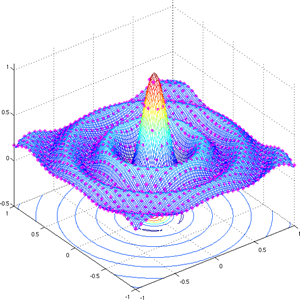
\includegraphics[scale=0.25]{../../img/sinc.PNG}}
在使用 Ubuntu 上的 Emacs org 生成 pdf 时默认的打开程序是 emacs,Emacs 打开 pdf 文档时非常慢。那么我想使用系统自带的  pdf 阅读器来查看,Ubuntu 系统自带的阅读器是 evince . 配置 emacs 使用 evince 打开 pdf 需要如下配置:

\lstset{language=Lisp,label= ,caption= ,captionpos=b,numbers=none}
\begin{lstlisting}
(setq org-file-apps
  (quote
   ((auto-mode . emacs)
    ("\\.pdf\\'" . "evince %s"))))
\end{lstlisting}
\end{document}
